\section{Method}
\label{sec:method}
This section describes \name, our framework for online context curation in
automated harness optimization. \name is built on the observation that prior
outer-loop systems either expose the full optimization history
monolithically~\cite{lee2026metaharness} or compress it into lossy
summaries~\cite{yang2024opro,lee2025feedback,agrawal2025gepa}. Neither static
exposure rule is optimal because the informativeness of a prior artifact
depends on the proposer's current iteration, recent edits, and observed
regressions. Instead, \name curates context through two composable strategies
that act at different granularities. The iteration-level strategy controls the
historical scope by selecting which prior rounds' artifacts to expose. The
file-level strategy can then reallocate read effort within the exposed
workspace by prioritizing files whose inspection has previously correlated
with productive edits. The file-level strategy is therefore not a standalone
replacement for iteration-level curation: by itself it does not decide which
prior iterations, traces, or candidate histories should enter the evidence
workspace.

\subsection{Problem Statement}
\label{sec:setting}
\textbf{Objective.}
A harness is a stateful program that wraps a fixed language model $M$ and determines what context $M$ sees at each step. Following~\cite{lee2026metaharness}, for a harness $H$ and task instance $x \sim X$, we execute a rollout trajectory $\tau \sim p_M(H, x)$ and score it with task-specific reward $r(\tau, x)$. The goal of automated harness optimization is to find
$$
H^* = \arg\max_H \mathbb{E}_{x \sim \mathcal{X}, \tau \sim p_M(H, x)} r(\tau, x).
$$

\textbf{Search loop with context curation.}
A run of the outer loop produces a sequence of evaluated candidates $\{(H_i, E_i)\}_{i=1}^t$, where $E_i$ bundles $H_i$'s source code, scores, and execution traces. We refer to the accumulated archive $D_t = \{\left(H_i, E_i\right)\}_{i \leq t}$ as the experience pool.
At each iteration $t$, the proposer $\mathcal{P}$ generates a new candidate conditioned on a curated context $C_t \subseteq D_t$:
\begin{equation}
H_{t+1} \sim P(\cdot \mid C_t),
\label{eq:search_loop}
\end{equation}
where $C_t = \mathcal{C}(D_t, s_t)$ is produced by a context curation policy $\mathcal{C}$ that selects which subset of $D_t$ to surface, and $s_t$ denotes the proposer's auxiliary state at iteration $t$ (e.g., current frontier, recent regressions).
After evaluation, $D_{t+1} = D_t \cup \{(H_{t+1}, E_{t+1})\}$. This formulation generalizes prior work: Lee et al.~\cite{lee2026metaharness} corresponds to direct filesystem access ($C_t = D_t$), while Agrawal et al.~\cite{agrawal2025gepa} and Yang et al.~\cite{yang2024opro} use static compression ($C_t = \phi(D_t)$ for some fixed $\phi$).

\subsection{\name}
\name is a closed-loop controller for sequential context selection. At each iteration $t$, it (i) maintains a state $s_t$ that summarizes past outcomes; (ii) computes scores $Q_t$ for candidate historical artifacts and files in $D_t$; (iii) applies a selection rule $\pi$ that maps these scores to the curated context $C_t$ in Eq.~\ref{eq:search_loop}; and (iv) after receiving the evaluation $E_{t+1}$, updates its state using a reward signal $\rho$ before the next proposal. The remainder of this section defines the shared state, scoring, selection, and update interface, and the following subsections instantiate it as the Progressive and bandit policies.

\textbf{State.} The controller's state has two components matching the two curation granularities, $s_t = (U_t, B_t)$. $U_t$ is an \emph{iteration-level summary} that tracks how recent proposals have performed against the Pareto frontier --- for instance, whether the last iteration was an improvement, or how many iterations have passed without one. $B_t$ holds \emph{per-file usage statistics}: for each file in the workspace, how often it has been read in past iterations and the cumulative reward attributed to those reads.

\textbf{Score.} Given $(D_t, s_t)$, \name estimates the expected value of surfacing each artifact for the next proposal, balanced against the inspection cost that the artifact would impose.

\textbf{Selection.} The selection rule converts these scores into an evidence workspace for the proposer. Depending on the instantiated strategy, this workspace may include labelled reference iterations, trace summaries, file-level hints, or a combination of these signals under a budget tier.

\textbf{Update.}  Once the evaluator returns its evaluation $E_{t+1}$, \name computes a scalar reward $\rho_{t+1}$ from $E_{t+1}$ that summarizes whether the new harness improved the search, updates the Pareto frontier, and refreshes $s_t \to s_{t+1}$. The refreshed state shapes the next round's scoring and selection. 

We instantiate the framework as two concrete policies operating at different granularities: an
\emph{iteration-level} policy that decides \emph{which prior rounds} to surface, and a \emph{file-level} policy that decides \emph{which files inside the exposed workspace} should receive priority.


\subsection{Iteration-level curation.}
\label{ssec:iteration}
Not every past iteration is equally informative, and its value changes with the proposer's current trajectory. For instance, after a successful update that extends the Pareto frontier, the proposer benefits most from seeing the recent winning candidates---reinforcing the direction that just
worked.  After a streak of failed attempts, however, the proposer needs a broader view: exposing earlier failures and their traces can reveal overlooked failure modes and inspire qualitatively different edits.  

We operationalize this intuition with a \emph{budget tier}
$b_t \in \{\texttt{low},\, \texttt{medium},\, \texttt{high}\}$ that controls how much of the experience pool $D_t$ is surfaced to the proposer.  Table~\ref{tab:budgets} specifies the context exposed at each tier: at \texttt{low}, the proposer sees only the single
best-scoring candidate and the worst-scoring one, together with
the most recent evaluation trace; at \texttt{high}, it receives
the full history.

\begin{table}[h]
\centering
\small
\caption{Budget tiers and the context they expose to the proposer. ``Reference iters'' determines which prior candidates are included; ``Trace scope'' controls how many recent per-task evaluation traces accompany each reference bundle.}
\begin{tabular}{@{}lccc@{}}
\toprule
 & \texttt{low} & \texttt{medium} & \texttt{high} \\
\midrule
Reference iters & best\,1 + worst & best\,3 + worst & full history \\
Trace scope     & last\,1         & last\,3         & all \\
\bottomrule
\end{tabular}
\label{tab:budgets}
\end{table}

The tier follows a \emph{progressive} schedule tied to the reward signal $\rho$ (Section~\ref{sec:method}).  The budget is initialized to \texttt{low}.  Whenever the proposer produces a candidate that fails to improve on the current Pareto frontier (i.e., $\rho_{t+1} \leq 0$), the tier is promoted by one level,
gradually widening the proposer's view of the experience pool.
When an improvement \emph{is} observed ($\rho_{t+1} > 0$), the tier resets to \texttt{low}, since the successful direction has been found and a lean context suffices to refine it. This schedule embodies a simple explore--exploit tradeoff: the controller starts conservative, broadens exposure only when progress stalls, and snaps back once a productive edit is discovered.

\begin{figure}[t]
  \centering
  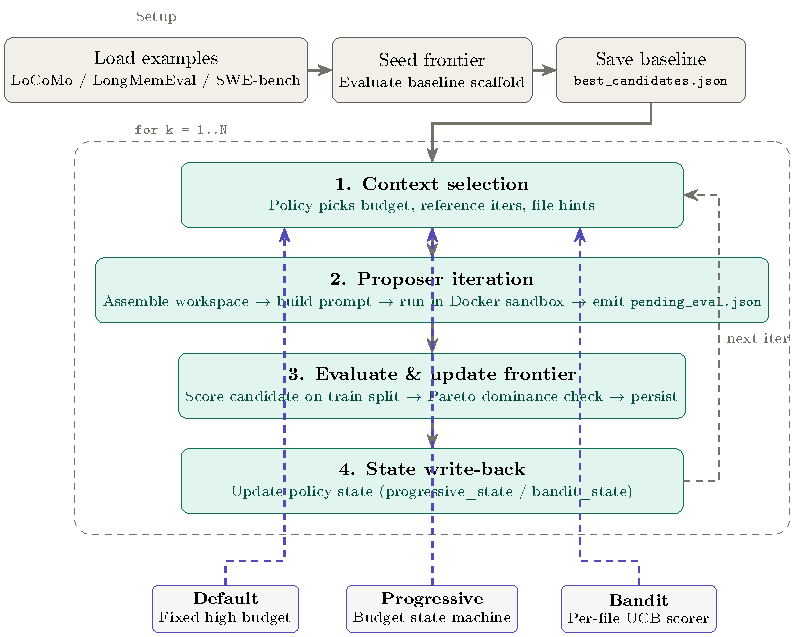
\includegraphics[width=\linewidth]{figures/system_overview.pdf}
  \vspace{-4pt}
  \caption{System overview. The setup phase evaluates baseline harnesses
  to seed the Pareto frontier. Each optimization iteration selects a
  context budget, assembles a sandboxed workspace, runs the proposer,
  evaluates the candidate, and writes back curation state. The loop
  repeats for $N$ iterations.}
  \label{fig:system_overview}
\end{figure}

\begin{figure}[t]
  \centering
  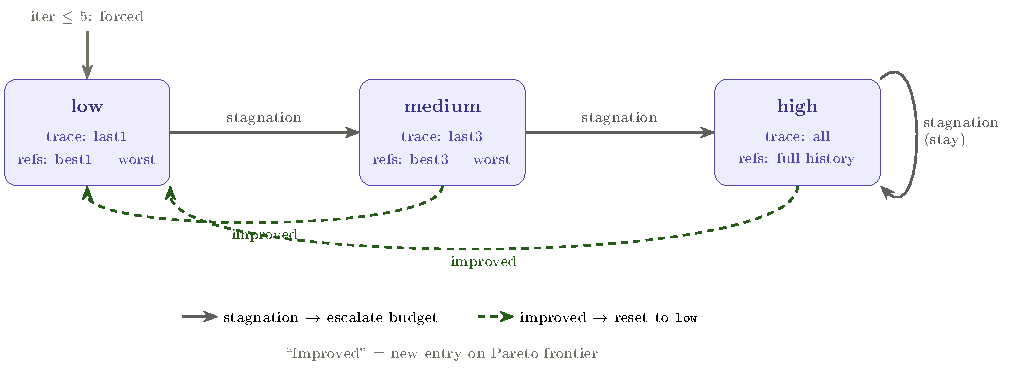
\includegraphics[width=0.92\linewidth]{figures/progressive_fsm.pdf}
  \caption{Progressive policy state machine. Solid arrows: budget
  escalation on stagnation (no new Pareto entry). Dashed arrows: reset
  to \texttt{low} on any improvement. The first $k_0\!=\!5$ iterations
  are forced to \texttt{low}.}
  \label{fig:progressive_fsm}
\end{figure}

\subsection{File-level Curation.}
\label{sec:bandit}
The file-level strategy is implemented as a bandit policy. It treats every readable file in the workspace as an arm of a multi-armed bandit (Figure~\ref{fig:bandit_flow}) and uses per-file utility estimates to construct a hot workspace that concentrates the proposer's attention on files whose past reads correlated with positive outcomes. This policy reallocates a bounded read budget rather than replacing historical-scope control: it is most natural after an evidence workspace has already been constructed, although the same scoring rule can be ablated under different reference-history budgets.

\paragraph{Reward signal.}
At the end of iteration~$k$, the harness computes a rolling $z$-score
reward from the candidate's passrate:
\begin{equation}
  r_k =
  \begin{cases}
    -\gamma/4 & \text{if no valid candidate was produced,} \\[2pt]
    \operatorname{clip}\!\bigl(
      (p_k - \hat\mu_k) \,/\, \hat\sigma_k,\;\pm\gamma
    \bigr) & \text{otherwise,}
  \end{cases}
  \label{eq:reward}
\end{equation}
where $p_k\!=\!p(h_k)$, and $\hat\mu_k,\hat\sigma_k$ are the mean and
standard deviation of passrates over the most recent~$W\!=\!8$
iterations (with $\hat\sigma_k \ge \sigma_{\min}$). The clip bound is
$\gamma\!=\!2$, and an iteration counts as a success when
$r_k > 0$. Normalizing against the recent window---rather than the
global best---lets a meaningful rebound during a stagnation stretch
still earn positive reward.

\paragraph{Per-file utility.}
After computing the reward, the harness records which files the proposer
read, wrote, and changed. For each file~$f$ in the discretionary read
pool (excluding a fixed set of always-included core files), the
policy score combines four components:
\begin{equation}
  S_f = \underbrace{0.7\,\Delta_f^{\text{bin}}
        + 0.3\,\Delta_f^{\text{rew}}}_{\text{utility}}
        - \underbrace{\lambda\,\log\!\bigl(1 + \bar\ell_f / L\bigr)}_{\text{cost}}
        + \underbrace{c\,\sqrt{\frac{\ln(k+1)}{n_f+1}}}_{\text{UCB bonus}},
  \label{eq:policy_score}
\end{equation}
where $\Delta_f^{\text{bin}}$ and $\Delta_f^{\text{rew}}$ are file~$f$'s
binary success rate and mean reward relative to the global mean (both
smoothed by a Beta prior of strength~$\alpha\!=\!2$), $\bar\ell_f$ is
the average number of lines read from~$f$, $n_f$ is the read count, and
$L\!=\!500$ is a line-count normalizer. The UCB bonus
($c\!=\!0.15$) ensures under-explored files are sampled before their
utility is written off, and the cost term ($\lambda\!=\!0.05$)
discourages over-reading large files.

\paragraph{Hot workspace and budget.}
Files are sorted by $S_f$; a fixed set of core files (target
scaffold source, base classes, summary files) is pinned, the top-8
scored files join the hot list (800-line read budget) and the
next-12 form the warm list (300-line budget). Together they
constitute the hot workspace surfaced to the proposer as advisory
hints---other files remain readable on demand. The budget tier is
\begin{equation}
  b_k =
  \begin{cases}
    \texttt{low}    & \text{if } k\!\le\!1 \text{ or no file stats,} \\
    \texttt{high}   & \text{if stagnation} \ge \theta\!=\!4, \\
    \texttt{medium} & \text{otherwise.}
  \end{cases}
  \label{eq:bandit_budget}
\end{equation}
Unlike the progressive policy, the bandit has no monotonic escalation
path: it stays at \texttt{medium} indefinitely as long as improvements
arrive before the stagnation window closes. At \texttt{high} budget
all prior iterations are referenced; at \texttt{medium} the bandit
selects up to five (iterations where hot files appeared, the top-3 by
passrate, and the last improving iteration); at \texttt{low} no raw
references are provided.

\begin{figure}[t]
  \centering
  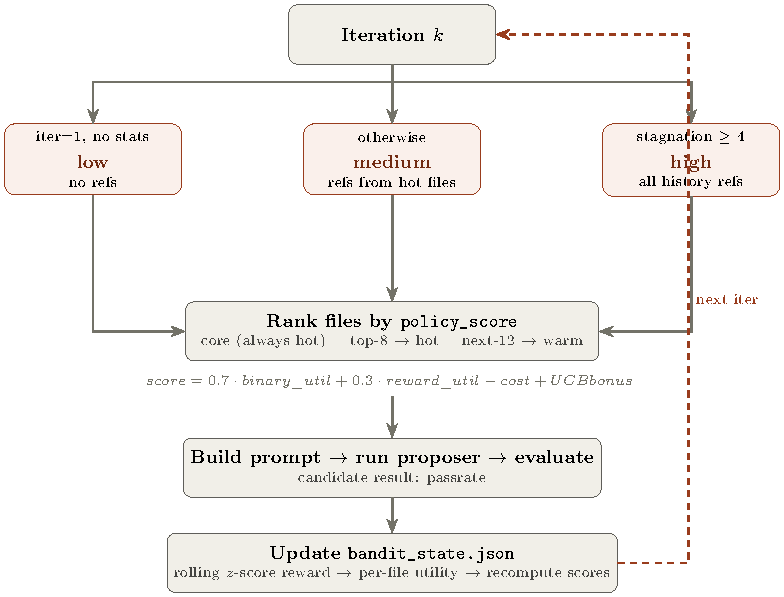
\includegraphics[width=0.88\linewidth]{figures/bandit_flow.pdf}
  \vspace{-4pt}
  \caption{Bandit policy decision flow. Each iteration starts with a
  budget decision based on stagnation count, ranks files by
  $S_f$~(Eq.~\ref{eq:policy_score}), runs the proposer, then feeds the
  reward (Eq.~\ref{eq:reward}) back to update per-file utility
  estimates.}
  \label{fig:bandit_flow}
\end{figure}
